\documentclass[11pt]{article}

\usepackage[margin=1in]{geometry}
\usepackage{amsmath,amssymb}
\usepackage{booktabs}
\usepackage{graphicx}
\usepackage{microtype}
\usepackage[hidelinks]{hyperref}
\usepackage{xcolor}
\usepackage{multirow}

\newcommand{\relL}{rel.\,$L_2$}
\newcommand{\B}{B}

\title{Does Risk-Aware Allocation Help Budgeted Correction of\\ Neural PDE Surrogates?\\
\large A negative result with a mechanistic explanation}

\author{Anonymous}
\date{Draft --- \today}

\begin{document}
\maketitle

\begin{abstract}
Neural surrogates for time-dependent PDEs can drift once they are rolled out
autoregressively. A natural remedy is to spend a fixed computational budget
replacing some surrogate steps with steps of the reference solver. Which steps
should receive the budget? We implement and evaluate a complete family of
allocators on three benchmarks (1D Burgers, 1D Allen--Cahn, 2D
advection--diffusion) under a single cost model in which one correction equals
one saved interval of the reference solver. Our main finding is negative and
consistent: a learned, conformally calibrated horizon-risk model does not beat a
training-free ensemble-disagreement ranking, fusion of the two adds nothing, and
a learned model of the \emph{counterfactual gain} of a correction is worse than
both. Even an oracle with access to the true one-step counterfactual gain loses
to the trivial schedule that spends the whole budget on the first $k$ steps once
the budget is large. We explain why with a policy-free measurement: the relative
value of a correction decays along the horizon on every benchmark (e.g.\ 0.236
to 0.119 on Burgers), and under distribution shift it becomes
\emph{anti-correlated} with the surrogate's own error (Spearman $-0.84$ on
shifted Burgers, $-0.84$ on advection--diffusion), so ranking steps by risk
systematically targets steps where correcting helps least. Budget compliance is
exact for ranked allocators, while the threshold baseline overspends by up to
$+0.90$ of the full-solver cost and the pacer underspends by up to $0.40$.
We report all negative and unstable outcomes, including seed counts and
CPU-only timing caveats.
\end{abstract}

\section{Introduction}

Operator-learning surrogates~\cite{li2021fno,lu2021deeponet,kovachki2023neural}
predict a PDE solution field at a fraction of the cost of a numerical solver.
When such a surrogate is used inside a long autoregressive rollout, small
one-step errors compound: on our benchmarks the mean relative error grows by
$24\times$ (Burgers), $78\times$ (Allen--Cahn) and $68\times$
(advection--diffusion) between one-step and full-horizon evaluation. A
practical remedy is hybrid execution: run the surrogate most of the time and
occasionally advance the reference solver from the current state.

This converts accuracy into an allocation problem. With a budget $B$ measured
as a fraction of the cost of running the reference solver over the whole
horizon, a step correction costs one unit and the policy may act $\lfloor BT
\rfloor$ times. The question we study is: \emph{does a learned, calibrated risk
model allocate this budget better than trivial heuristics?}

We built BRACE (Budgeted Risk-Adaptive Correction Engine) to answer this with a
controlled comparison rather than a demonstration. The design had three
properties we consider necessary for a credible answer:

\begin{enumerate}
\item \textbf{One cost model, exactly enforced.} One step correction costs one
  saved interval; a window of $W$ costs $W$; re-anchoring from $u_0$ to step $t$
  costs $t+1$. Top-$k$ allocation with $k=\lfloor BT\rfloor$ makes realised cost
  equal declared cost by construction. We verify this and report the deviation
  for every run.
\item \textbf{Trivial baselines that could win.} Uniform spacing, front-loading
  (\texttt{early}), static residual thresholding, online quantile pacing, and a
  training-free ensemble-disagreement ranking are all included. Front-loading in
  particular is the baseline that a risk-aware method must beat to justify
  itself, and it is not a straw man.
\item \textbf{Oracles for the objective.} We include an oracle that ranks steps
  by their true one-step error and an oracle that ranks them by the true
  \emph{counterfactual gain} of a correction. If a learned model cannot
  approach its own oracle, the objective or the signal is at fault, not the
  fit.
\end{enumerate}

\paragraph{What we found.} Budgeted correction works: on Burgers-1D, test error
drops from 0.0611 (surrogate only) to 0.0178--0.0215 at $B=0.4$ depending on the
allocator. But the sophistication of the allocator does not pay. Ensemble
disagreement, which requires no training beyond the ensemble itself, matches or
beats the calibrated horizon-risk model at $B=0.1/0.2$ on all three benchmarks;
front-loading is best or tied-best at $B=0.4$. The learned gain model is worse
than ensemble ranking in-distribution and degenerates to front-loading under
severe shift, where its predictions become constant. The gain oracle itself loses to
front-loading at large budgets, so the greedy one-step objective is the wrong
objective, not merely badly estimated.

We then measure the mechanism without reference to any policy. The relative
gain of a correction, $\mathbb{E}[(e_{\text{neural}}-e_{\text{corrected}})/e_{\text{neural}}]$,
decays along the horizon and, under shift, is strongly \emph{negatively}
correlated with the surrogate's own error. Ranking by risk thus selects the
steps where a correction is least useful. This single measurement explains the
allocation results, the failure of the gain oracle at large budgets, and why
front-loading is hard to beat.

\paragraph{Contributions.}
\begin{itemize}
\item A budget-exact hybrid-execution harness with a single comparable cost
  metric and an audit of realised versus declared cost for every policy
  (Section~\ref{sec:cost}, Table~\ref{tab:audit}).
\item A controlled comparison of the full allocator family
  (Table~\ref{tab:policies}), including two oracles, on three PDEs and three
  distributional settings (Section~\ref{sec:results}).
\item A negative result for learned risk- and gain-based allocation, with
  oracles that bound what any allocator of that family could achieve
  (Sections~\ref{sec:allocation}--\ref{sec:gain}).
\item A policy-free mechanistic explanation: horizon decay and error--gain
  anti-correlation under shift (Section~\ref{sec:mechanism}).
\item Ablations showing that ensemble disagreement is the only component that
  matters, and that several components of the risk model actively hurt
  (Section~\ref{sec:ablation}).
\end{itemize}

\section{Related work}

\paragraph{Neural operators and hybrid solvers.} Fourier neural
operators~\cite{li2021fno} and DeepONet~\cite{lu2021deeponet} learn maps between
function spaces; \cite{kovachki2023neural} gives a unified account. Learned
discretisations~\cite{barsinai2019learning} and solver-in-the-loop
training~\cite{um2020solver} also combine learned components with numerical
integrators, but target training-time correction rather than test-time budget
allocation. Our question is complementary: given a fixed surrogate, where should
solver work be spent?

\paragraph{Uncertainty for scientific surrogates.} Deep
ensembles~\cite{lakshminarayanan2017deep} are a strong, cheap baseline for
epistemic uncertainty, and calibration of predictive
probabilities~\cite{guo2017calibration} is routinely miscalibrated without
explicit treatment. Split conformal prediction~\cite{vovk2005algorithmic,
angelopoulos2021gentle} gives distribution-free intervals under exchangeability;
we measure rather than assume coverage under shift. Uncertainty quantification
for scientific machine learning is surveyed
in~\cite{psaros2023uncertainty}.

\paragraph{Benchmarks.} PDEBench~\cite{takamoto2022pdebench} standardises
surrogate benchmarks; we use smaller, purpose-built datasets so that the exact
reference solver is available at every step for counterfactual measurements.

\section{Setting and cost model}
\label{sec:cost}

Let $u_t\in\mathbb{R}^{n}$ be the state at saved interval $t$, $t=0,\dots,T$.
The reference solver advances one saved interval at cost $1$; a full simulation
costs $T$. A surrogate ensemble $\{g_m\}_{m=1}^{M}$ predicts the increment
$u_{t+1}=u_t+\frac1M\sum_m g_m(u_t)$, so the identity path is exact and the
network models only a local correction.

A budget $B\in(0,1]$ permits $\lfloor BT\rfloor$ step corrections per
trajectory. We use three correction primitives:
\begin{itemize}
\item \textbf{step}: integrate the reference solver one interval from the
  current state, cost $1$;
\item \textbf{window} of width $W$: integrate $W$ intervals, cost $W$, with
  starts restricted to $t\ge W-1$ so no window is truncated;
\item \textbf{re-anchor} at $t$: integrate $t+1$ intervals from $u_0$, cost
  $t+1$.
\end{itemize}
``Running the solver'' is $B=1$. Budget accounting covers reference-solver work
only. Planning (feature extraction, scoring) is reported separately in
Section~\ref{sec:compute} and is not charged to the budget; we flag this because
it favours our method.

\section{Method}

\subsection{Online risk features}
At each step, before committing to the surrogate prediction, we compute nine
features from quantities available online: mean and maximum ensemble standard
deviation, relative PDE residual of the ensemble mean, a conservation
deviation, the magnitude of the predicted update, temporal inconsistency between
the surrogate and PDE-predicted increments, two exponentially weighted history
terms, and normalised time. No ground-truth state is used.

\subsection{Risk and calibration}
Two ridge/logistic models are fit on validation trajectories only: a \emph{step}
model for one-step error and failure probability ($e>\tau$, $\tau=0.05$), and a
\emph{horizon} model for the discounted future error
$\sum_{s\ge t}\gamma^{s-t}e_s$ with $\gamma=0.95$. Split conformal calibration
on validation residuals yields an interval for one-step error at nominal
coverage $1-\alpha$ with $\alpha=0.1$. Exchangeability is assumed for the
guarantee and tested empirically on shifted splits
(Section~\ref{sec:ood}).

\subsection{Gain model}
Risk asks whether a step is bad; a correction's value asks whether integrating
the solver \emph{from the current state} reduces the error. On validation data
we compute the counterfactual gain $e_{\text{neural}}-e_{\text{corrected}}$ by
advancing the reference solver from each uncorrected surrogate state, and fit a
ridge model of the \emph{relative} gain
$g=\mathrm{clip}((e_{\text{neural}}-e_{\text{corrected}})/e_{\text{neural}},0,1)$
on the nine online features. The allocation score is
$\hat{g}\cdot\hat{e}$ (predicted relative gain times predicted error). Gain
labels require validation ground truth and solver work, so fitting is an
offline cost and is not charged to the test budget.

\subsection{Controllers}
Table~\ref{tab:policies} lists the policies. Budget-exact policies take the
per-trajectory top-$k$ scores with $k=\lfloor BT\rfloor$, excluding overlapping
windows and truncated windows. \texttt{brace\_combo} fuses standardised horizon
risk and standardised ensemble disagreement with fixed equal weights chosen a
priori, not tuned on test. \texttt{oracle} ranks by true one-step error;
\texttt{oracle\_gain} ranks by the true counterfactual gain computed on the
uncorrected rollout.

\begin{table}[t]
\centering
\small
\begin{tabular}{lll}
\toprule
Policy & Score & Budget-aware \\
\midrule
\texttt{neural} & none & n/a \\
\texttt{numerical} & every step & cost 1.0 \\
\texttt{fixed} & static threshold on validation residual quantile & no \\
\texttt{adaptive} & online quantile with cumulative pacing & partially \\
\texttt{uniform} & evenly spaced steps & exact \\
\texttt{early} & first $k$ steps & exact \\
\texttt{ranked\_residual} & relative PDE residual & exact \\
\texttt{ranked\_ensemble} & ensemble disagreement & exact \\
\texttt{ranked\_calibrated} & step risk model & exact \\
\texttt{brace} & horizon risk model & exact \\
\texttt{brace\_combo} & horizon risk $+$ disagreement (equal weights) & exact \\
\texttt{gain\_ranked} & predicted relative gain $\times$ predicted error & exact \\
\texttt{oracle\_gain} & true counterfactual gain & exact \\
\texttt{oracle} & true one-step error & exact \\
\texttt{reanchor} & re-integrate from $u_0$ to the chosen step & exact \\
\bottomrule
\end{tabular}
\caption{Allocators. ``Exact'' means realised cost equals the declared budget
by construction (verified in Table~\ref{tab:audit}).}
\label{tab:policies}
\end{table}

\subsection{Metrics and statistics}
We report mean relative $L_2$ error over trajectories and horizon
(\relL), the fraction of (trajectory, step) pairs with relative error above
$\tau=0.1$, the fraction of trajectories with mean relative error above $1$
(divergence), and realised cost. Seed-level 95\% intervals use Student-$t$ with
$n-1$ degrees of freedom. Paired comparisons over identical trajectories use a
$5000$-resample paired bootstrap~\cite{efron1993bootstrap}, a paired $t$-test, Wilcoxon, and Cohen's
$d_z$. With a single seed we report point estimates and per-trajectory paired
intervals, not seed intervals.

\section{Experiments}

\paragraph{Benchmarks.} 1D Burgers ($\nu\in[0.005,0.02]$, $n=128$, $T=100$
intervals of $0.02$), 1D Allen--Cahn ($\epsilon=0.01$, $n=128$, $T=100$
intervals of $0.01$), and 2D advection--diffusion ($n=64$, evaluated on a
$32\times32$ Fourier truncation, $T=100$ intervals of $0.02$). The 2D equation
is linear and solved exactly by its Fourier symbol, so reference steps are not
limited by temporal discretisation error.

\paragraph{Splits.} \texttt{train} fits surrogate parameters, \texttt{val} fits
risk and gain models and conformal calibration, \texttt{test} is in-distribution,
\texttt{ood\_param} shifts viscosity or transport speed outside the training
range, and \texttt{ood\_ic} shifts initial-condition length scale and amplitude.
Datasets carry SHA-256 checksums; an audit verifies 15 datasets, zero checksum
mismatches, zero initial-condition leakage between splits, and zero non-finite
fields.

\paragraph{Surrogates.} FNO with residual (increment) output: width 32, 32 modes,
4 layers for 1D; width 16, 8 modes, 3 layers for 2D. Ensembles of three members
(Burgers, Allen--Cahn) and two members (advection--diffusion), trained with
different seeds. A DeepONet with one member is included as an
architecture-agnosticism check, not as a comparison. Burgers test uses two
surrogate seeds; the other benchmarks use one.

\section{Results}
\label{sec:results}

\subsection{Correction reduces error substantially}
On Burgers test the surrogate-only error is 0.0611. At $B=0.4$ every ranked
policy is below 0.035, and the best is 0.0178, a 71\% reduction at 40\% of
full-solver cost. Table~\ref{tab:main} and Figure~\ref{fig:pareto} report the grid.

\begin{table*}[t]
\centering
\footnotesize
\setlength{\tabcolsep}{4pt}
\begin{tabular}{lllrrr}
\toprule
Benchmark & Split & Policy & $B=0.1$ & $B=0.2$ & $B=0.4$ \\
\midrule
burgers1d & test & surrogate only & 0.061 & 0.061 & 0.061 \\
burgers1d & test & uniform & 0.041/0.10 & 0.031/0.20 & 0.021/0.40 \\
burgers1d & test & early & 0.055/0.10 & 0.042/0.20 & 0.018/0.40 \\
burgers1d & test & residual-ranked & 0.043/0.10 & 0.036/0.20 & 0.027/0.40 \\
burgers1d & test & ensemble-ranked & 0.039/0.10 & 0.030/0.20 & 0.019/0.40 \\
burgers1d & test & BRACE & 0.040/0.10 & 0.032/0.20 & 0.021/0.40 \\
burgers1d & test & BRACE-fusion & 0.039/0.10 & 0.031/0.20 & 0.020/0.40 \\
burgers1d & test & gain-ranked & 0.043/0.10 & 0.036/0.20 & 0.027/0.40 \\
burgers1d & test & gain oracle & 0.041/0.10 & 0.033/0.20 & 0.024/0.40 \\
burgers1d & test & oracle & 0.048/0.10 & 0.043/0.20 & 0.035/0.40 \\
\midrule
allencahn1d & test & surrogate only & 0.008 & 0.008 & 0.008 \\
allencahn1d & test & uniform & 0.007/0.10 & 0.006/0.20 & 0.005/0.40 \\
allencahn1d & test & early & 0.006/0.10 & 0.005/0.20 & 0.003/0.40 \\
allencahn1d & test & residual-ranked & 0.007/0.10 & 0.007/0.20 & 0.006/0.40 \\
allencahn1d & test & ensemble-ranked & 0.006/0.10 & 0.005/0.20 & 0.003/0.40 \\
allencahn1d & test & BRACE & 0.007/0.10 & 0.006/0.20 & 0.004/0.40 \\
allencahn1d & test & BRACE-fusion & 0.006/0.10 & 0.005/0.20 & 0.003/0.40 \\
allencahn1d & test & gain-ranked & 0.007/0.10 & 0.006/0.20 & 0.004/0.40 \\
allencahn1d & test & gain oracle & 0.007/0.10 & 0.006/0.20 & 0.005/0.40 \\
allencahn1d & test & oracle & 0.007/0.10 & 0.007/0.20 & 0.006/0.40 \\
\midrule
advection2d & test & surrogate only & 0.554 & 0.554 & 0.554 \\
advection2d & test & uniform & 0.507/0.10 & 0.459/0.20 & 0.356/0.40 \\
advection2d & test & early & 0.453/0.10 & 0.361/0.20 & 0.207/0.40 \\
advection2d & test & residual-ranked & 0.483/0.10 & 0.417/0.20 & 0.305/0.40 \\
advection2d & test & ensemble-ranked & 0.469/0.10 & 0.393/0.20 & 0.255/0.40 \\
advection2d & test & BRACE & 0.486/0.10 & 0.417/0.20 & 0.295/0.40 \\
advection2d & test & BRACE-fusion & 0.483/0.10 & 0.411/0.20 & 0.281/0.40 \\
advection2d & test & gain-ranked & 0.472/0.10 & 0.406/0.20 & 0.287/0.40 \\
advection2d & test & gain oracle & 0.454/0.10 & 0.366/0.20 & 0.218/0.40 \\
advection2d & test & oracle & 0.551/0.10 & 0.539/0.20 & 0.488/0.40 \\
\midrule
\bottomrule
\end{tabular}

\caption{In-distribution results: relative $L_2$ error / realised cost.
`Surrogate only' is the uncorrected rollout. Burgers is a two-seed mean; the
other rows are single-seed point estimates. The full grid over all splits and
all policies, with seed intervals, is in the supplement.}
\label{tab:main}
\end{table*}

\begin{figure}[t]
\centering
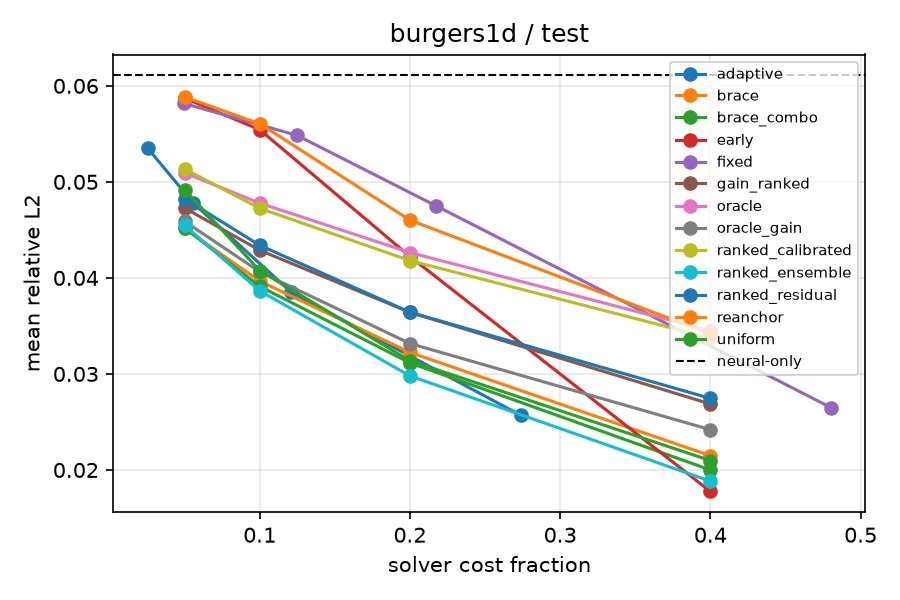
\includegraphics[width=0.48\textwidth]{figures/pareto_burgers.png}
\hfill
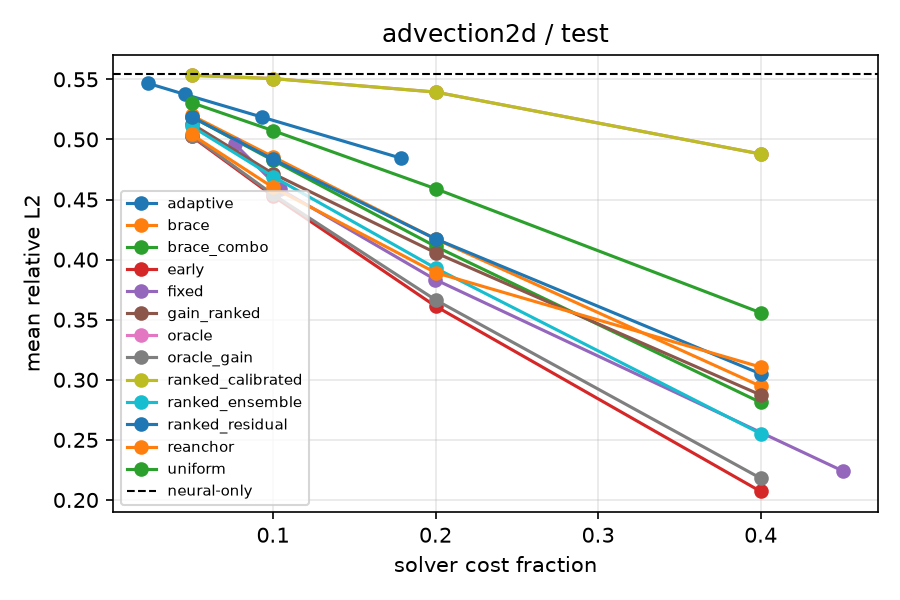
\includegraphics[width=0.48\textwidth]{figures/pareto_advection.png}
\caption{Error versus realised cost on Burgers-1D (left) and
advection--diffusion-2D (right). The frontier is populated by training-free
schedules and ensemble ranking; the risk-based allocators sit on top of them
rather than below.}
\label{fig:pareto}
\end{figure}

\subsection{The learned risk model does not beat a training-free score}
\label{sec:allocation}

At every budget the training-free ensemble-disagreement ranking is never
significantly worse than the calibrated horizon-risk model, and at $B=0.1/0.2$
it is better on all three in-distribution benchmarks: 0.0387/0.0298 on Burgers
test (vs 0.0397/0.0322), 0.0062/0.0050 on Allen--Cahn (vs 0.0067/0.0059), and
0.4691/0.3929 on advection--diffusion (vs 0.4856/0.4172). On Burgers test the
paired difference for the horizon-risk model against ensemble ranking is
$+0.0024$ at $B=0.2$ (seed-level 95\% half-width $0.0093$, $d_z=0.35$, one of
two seeds significant) and $+0.0027$ at $B=0.4$ (half-width $0.0020$,
$d_z=0.43$, both seeds significant). Across the in-distribution grid the only
place the risk model is nominally ahead is $B=0.05$ on Burgers, by $0.0004$ with
a paired half-width of $0.002$, i.e.\ not distinguishable. Fusing the two
(\texttt{brace\_combo}) does not help: on Burgers test its paired differences
against ensemble ranking are $-0.0003$, $+0.0005$, $+0.0014$ and $+0.0012$ at
$B=0.05,0.1,0.2,0.4$; none is a significant improvement, and the last two are
significantly worse on at least one seed.

At $B=0.4$ front-loading is best or tied-best on all three benchmarks among
budget-feasible policies (0.0178 Burgers, 0.0029 Allen--Cahn tied with ensemble
ranking, 0.2071 advection--diffusion), and on advection--diffusion it is best at
every budget (0.4530/0.3613/0.2071 at $B=0.1/0.2/0.4, versus
0.4691/0.3929/0.2552 for ensemble ranking). This is the first indication that
\emph{when} the budget is spent dominates \emph{how} it is ranked.

\subsection{Learning the gain of a correction makes things worse}
\label{sec:gain}

The gain model is worse than ensemble ranking at every budget on all three
in-distribution benchmarks (Burgers test $+0.0018$ to $+0.0080$; Allen--Cahn
$+0.0002$ to $+0.0014$; advection--diffusion $+0.0021$ to $+0.0322$) and on
Burgers \texttt{ood\_param} by $+0.0140$ to $+0.0510$ (both seeds significant,
$d_z$ up to 2.07). It has one apparent success and it is not one: on severely
shifted advection--diffusion it beats ensemble ranking (0.560 vs 0.650 at
$B=0.4$), but its predicted scores become nearly constant under shift, so the
top-$k$ tie-break selects the first $k$ steps; on the
\texttt{ood\_ic} split its error equals the \texttt{early} schedule to four
decimals at all three budgets. The gain
model has collapsed, not improved.

Decisively, the gain \emph{oracle} loses to front-loading at large budgets:
0.0242 vs 0.0178 (Burgers), 0.0046 vs 0.0029 (Allen--Cahn), 0.2181 vs 0.2071
(advection--diffusion) at $B=0.4$. Since the oracle has the true one-step
counterfactual gain, the greedy one-step objective itself is inadequate. A
correction changes the state on which all later predictions are made, and the
one-step gain does not see that benefit.

\subsection{Mechanism: value decays with horizon, and inverts under shift}
\label{sec:mechanism}

We measure, independently of any policy, the counterfactual relative gain at
every step of an uncorrected held-out rollout
(Table~\ref{tab:decay}). Two regularities are consistent across benchmarks.

\begin{table}[t]
\centering
\small
\begin{tabular}{lccc}
\toprule
Benchmark / split & relative gain (first $\to$ last decile) & harm rate & Spearman(pre-error, gain) \\
\midrule
Burgers test & $0.236\to0.119$ & 0.3\% & $+0.008$ \\
Burgers \texttt{ood\_param} & $0.195\to0.024$ & 3.7\% & $-0.843$ \\
Allen--Cahn test & $0.155\to0.015$ & 0.0\% & $-0.665$ \\
Advection--diffusion test & $0.149\to0.009$ & 0.1\% & $-0.842$ \\
\bottomrule
\end{tabular}
\caption{Correction value versus horizon position and versus surrogate error.
Harm rate is the fraction of corrected steps whose error increases.}
\label{tab:decay}
\end{table}

First, value decays monotonically along the horizon. A correction applied to a
state that has already drifted integrates the PDE from the wrong initial
condition, so the resulting field is a valid solution of the PDE but not of the
original problem. Second, in-distribution the surrogate's error carries almost
no information about relative gain (Spearman $+0.008$ on Burgers); under shift
the correlation becomes strongly negative. The highest-error steps are the ones
where a correction helps least. This is exactly why the true-error oracle is the
\emph{worst} ranked allocator on advection--diffusion (0.488 at $B=0.4$ vs 0.207
for front-loading), and why any risk-based ranker is structurally handicapped
relative to spending early.

\subsection{Out-of-distribution behaviour}
\label{sec:ood}

Table~\ref{tab:ood_param} and Table~\ref{tab:ood_ic} report the shifted splits.
At $B=0.4$ front-loading is best or tied-best on Burgers \texttt{ood\_ic}
(0.067), both Allen--Cahn shifts (0.012, 0.003), and both
advection--diffusion shifts (0.625, 0.560); the exception is Burgers
\texttt{ood\_param}, where ensemble ranking is best (0.108 vs 0.121). At
$B=0.1/0.2$, ranking policies remain best on the Burgers shifts, while
front-loading ties ensemble ranking on Allen--Cahn and is best among
budget-feasible policies on advection--diffusion. The static-threshold
baseline is best on several shifts only by spending far more than the declared
budget.

\begin{table*}[t]
\centering
\footnotesize
\setlength{\tabcolsep}{4pt}
\begin{tabular}{lllrrr}
\toprule
Benchmark & Split & Policy & $B=0.1$ & $B=0.2$ & $B=0.4$ \\
\midrule
burgers1d & ood\_param & surrogate only & 0.220 & 0.220 & 0.220 \\
burgers1d & ood\_param & uniform & 0.198/0.10 & 0.182/0.20 & 0.159/0.40 \\
burgers1d & ood\_param & early & 0.212/0.10 & 0.185/0.20 & 0.121/0.40 \\
burgers1d & ood\_param & residual-ranked & 0.195/0.10 & 0.180/0.20 & 0.151/0.40 \\
burgers1d & ood\_param & ensemble-ranked & 0.184/0.10 & 0.160/0.20 & 0.108/0.40 \\
burgers1d & ood\_param & BRACE & 0.186/0.10 & 0.163/0.20 & 0.116/0.40 \\
burgers1d & ood\_param & BRACE-fusion & 0.185/0.10 & 0.160/0.20 & 0.110/0.40 \\
burgers1d & ood\_param & gain-ranked & 0.198/0.10 & 0.184/0.20 & 0.159/0.40 \\
burgers1d & ood\_param & gain oracle & 0.180/0.10 & 0.154/0.20 & 0.109/0.40 \\
burgers1d & ood\_param & oracle & 0.212/0.10 & 0.206/0.20 & 0.194/0.40 \\
\midrule
allencahn1d & ood\_param & surrogate only & 0.032 & 0.032 & 0.032 \\
allencahn1d & ood\_param & uniform & 0.029/0.10 & 0.026/0.20 & 0.020/0.40 \\
allencahn1d & ood\_param & early & 0.026/0.10 & 0.021/0.20 & 0.012/0.40 \\
allencahn1d & ood\_param & residual-ranked & 0.031/0.10 & 0.029/0.20 & 0.024/0.40 \\
allencahn1d & ood\_param & ensemble-ranked & 0.026/0.10 & 0.021/0.20 & 0.012/0.40 \\
allencahn1d & ood\_param & BRACE & 0.030/0.10 & 0.027/0.20 & 0.021/0.40 \\
allencahn1d & ood\_param & BRACE-fusion & 0.028/0.10 & 0.024/0.20 & 0.017/0.40 \\
allencahn1d & ood\_param & gain-ranked & 0.028/0.10 & 0.025/0.20 & 0.020/0.40 \\
allencahn1d & ood\_param & gain oracle & 0.027/0.10 & 0.021/0.20 & 0.013/0.40 \\
allencahn1d & ood\_param & oracle & 0.032/0.10 & 0.031/0.20 & 0.027/0.40 \\
\midrule
advection2d & ood\_param & surrogate only & 1.195 & 1.195 & 1.195 \\
advection2d & ood\_param & uniform & 1.166/0.10 & 1.136/0.20 & 1.039/0.40 \\
advection2d & ood\_param & early & 1.054/0.10 & 0.912/0.20 & 0.625/0.40 \\
advection2d & ood\_param & residual-ranked & 1.146/0.10 & 1.091/0.20 & 0.976/0.40 \\
advection2d & ood\_param & ensemble-ranked & 1.097/0.10 & 1.001/0.20 & 0.793/0.40 \\
advection2d & ood\_param & BRACE & 1.161/0.10 & 1.115/0.20 & 0.998/0.40 \\
advection2d & ood\_param & BRACE-fusion & 1.160/0.10 & 1.116/0.20 & 0.998/0.40 \\
advection2d & ood\_param & gain-ranked & 1.076/0.10 & 0.918/0.20 & 0.626/0.40 \\
advection2d & ood\_param & gain oracle & 1.054/0.10 & 0.912/0.20 & 0.649/0.40 \\
advection2d & ood\_param & oracle & 1.206/0.10 & 1.210/0.20 & 1.186/0.40 \\
\midrule
\bottomrule
\end{tabular}

\caption{Parameter shift: relative $L_2$ error / realised cost. The `fixed'
threshold baseline is omitted because its realised cost is not the declared
budget (Table~\ref{tab:audit}); on several of these splits it reaches cost
$1.00$.}
\label{tab:ood_param}
\end{table*}

\begin{table*}[t]
\centering
\footnotesize
\setlength{\tabcolsep}{4pt}
\begin{tabular}{lllrrr}
\toprule
Benchmark & Split & Policy & $B=0.1$ & $B=0.2$ & $B=0.4$ \\
\midrule
burgers1d & ood\_ic & surrogate only & 0.175 & 0.175 & 0.175 \\
burgers1d & ood\_ic & uniform & 0.131/0.10 & 0.107/0.20 & 0.075/0.40 \\
burgers1d & ood\_ic & early & 0.157/0.10 & 0.131/0.20 & 0.067/0.40 \\
burgers1d & ood\_ic & residual-ranked & 0.148/0.10 & 0.130/0.20 & 0.100/0.40 \\
burgers1d & ood\_ic & ensemble-ranked & 0.130/0.10 & 0.106/0.20 & 0.076/0.40 \\
burgers1d & ood\_ic & BRACE & 0.137/0.10 & 0.113/0.20 & 0.089/0.40 \\
burgers1d & ood\_ic & BRACE-fusion & 0.136/0.10 & 0.112/0.20 & 0.084/0.40 \\
burgers1d & ood\_ic & gain-ranked & 0.135/0.10 & 0.113/0.20 & 0.088/0.40 \\
burgers1d & ood\_ic & gain oracle & 0.133/0.10 & 0.108/0.20 & 0.077/0.40 \\
burgers1d & ood\_ic & oracle & 0.155/0.10 & 0.140/0.20 & 0.115/0.40 \\
\midrule
allencahn1d & ood\_ic & surrogate only & 0.016 & 0.016 & 0.016 \\
allencahn1d & ood\_ic & uniform & 0.013/0.10 & 0.012/0.20 & 0.008/0.40 \\
allencahn1d & ood\_ic & early & 0.010/0.10 & 0.007/0.20 & 0.003/0.40 \\
allencahn1d & ood\_ic & residual-ranked & 0.010/0.10 & 0.007/0.20 & 0.004/0.40 \\
allencahn1d & ood\_ic & ensemble-ranked & 0.010/0.10 & 0.007/0.20 & 0.003/0.40 \\
allencahn1d & ood\_ic & BRACE & 0.010/0.10 & 0.007/0.20 & 0.004/0.40 \\
allencahn1d & ood\_ic & BRACE-fusion & 0.010/0.10 & 0.007/0.20 & 0.004/0.40 \\
allencahn1d & ood\_ic & gain-ranked & 0.010/0.10 & 0.007/0.20 & 0.004/0.40 \\
allencahn1d & ood\_ic & gain oracle & 0.010/0.10 & 0.007/0.20 & 0.003/0.40 \\
allencahn1d & ood\_ic & oracle & 0.014/0.10 & 0.012/0.20 & 0.009/0.40 \\
\midrule
advection2d & ood\_ic & surrogate only & 1.289 & 1.289 & 1.289 \\
advection2d & ood\_ic & uniform & 1.204/0.10 & 1.133/0.20 & 0.988/0.40 \\
advection2d & ood\_ic & early & 1.050/0.10 & 0.863/0.20 & 0.560/0.40 \\
advection2d & ood\_ic & residual-ranked & 1.050/0.10 & 0.863/0.20 & 0.560/0.40 \\
advection2d & ood\_ic & ensemble-ranked & 1.076/0.10 & 0.903/0.20 & 0.650/0.40 \\
advection2d & ood\_ic & BRACE & 1.155/0.10 & 1.021/0.20 & 0.732/0.40 \\
advection2d & ood\_ic & BRACE-fusion & 1.155/0.10 & 1.020/0.20 & 0.728/0.40 \\
advection2d & ood\_ic & gain-ranked & 1.050/0.10 & 0.863/0.20 & 0.560/0.40 \\
advection2d & ood\_ic & gain oracle & 1.055/0.10 & 0.925/0.20 & 0.725/0.40 \\
advection2d & ood\_ic & oracle & 1.245/0.10 & 1.208/0.20 & 1.115/0.40 \\
\midrule
\bottomrule
\end{tabular}

\caption{Initial-condition shift: relative $L_2$ error / realised cost.}
\label{tab:ood_ic}
\end{table*}

\paragraph{Calibration fails, compliance holds.} Empirical conformal coverage at
nominal 0.9 is 0.929/0.944 on Burgers test (two seeds) but 0.430/0.490 on
\texttt{ood\_param} and 0.585 on \texttt{ood\_ic}; for advection--diffusion it
falls to 0.045 and 0.007. Upper-bound coverage is 0.96--1.00 on every split
except Burgers \texttt{ood\_param}, where it falls to 0.44--0.50; on that split
the interval is unsafe, not merely miscalibrated (full risk table in the
supplement). Budget compliance
is unaffected for ranked policies because it is enforced by construction
(Table~\ref{tab:audit}), but the achievable benefit shrinks: on
advection--diffusion \texttt{ood\_param} the surrogate error is 1.195 and the
best budgeted correction at $B=0.4$ is 0.625; on \texttt{ood\_ic} the
corresponding numbers are 1.289 and 0.560.

\paragraph{Threshold baselines silently abandon their budget.}
Table~\ref{tab:audit} audits declared versus realised cost over all main runs.
Every ranked policy deviates by less than $0.001$. The static-threshold baseline
overspends in 19 of 30 runs by up to $+0.900$ (and underspends in 4 by up to
$0.089$); under shift it reaches cost $1.000$ on seven runs, and on two of them
its error is at machine precision, i.e.\ it becomes the reference solver while
claiming a budget of $0.1$--$0.4$. The paced adaptive baseline underspends in
23 of 30 runs by up to $0.400$, leaving budget unused. Both behaviours are easy
to miss if only error is reported.

\begin{table}[t]
\centering
\small
\begin{tabular}{lrrrrr}
\toprule
Policy & runs & over & under & max $\Delta$ & min $\Delta$ \\
\midrule
fixed & 20 & 11 & 4 & +0.699 & -0.089 \\
adaptive & 20 & 0 & 13 & +0.006 & -0.222 \\
uniform & 14 & 0 & 0 & +0.000 & +0.000 \\
early & 14 & 0 & 0 & +0.000 & +0.000 \\
residual-ranked & 20 & 0 & 0 & +0.000 & +0.000 \\
ensemble-ranked & 20 & 0 & 0 & +0.000 & +0.000 \\
calib.-ranked & 20 & 0 & 0 & +0.000 & +0.000 \\
BRACE & 20 & 0 & 0 & +0.000 & +0.000 \\
BRACE-fusion & 20 & 0 & 0 & +0.000 & +0.000 \\
oracle & 20 & 0 & 0 & +0.000 & +0.000 \\
reanchor & 20 & 0 & 0 & +0.000 & +0.000 \\
\bottomrule
\end{tabular}

\caption{Declared versus realised cost across all main runs. `over'/'under'
count runs deviating by more than $0.02$.}
\label{tab:audit}
\end{table}

\subsection{Ablations}
\label{sec:ablation}

On Burgers test, seed 0, removing the ensemble (single member) degrades the
horizon-risk model from 0.0324 to 0.0416 at $B=0.2$ and from 0.0205 to 0.0267 at
$B=0.4$ ($+28\%$, $+31\%$). Restricting to residual features costs $+12\%$ and
$+30\%$. Every other component is within noise, and several removals improve the
model: dropping the temporal-consistency feature gives 0.0300/0.0185, and
$\gamma=0.99$ gives 0.0333/0.0182. The components of the risk model beyond
ensemble information do not earn their place.

\subsection{Correction granularity}
At matched budget, step corrections beat window corrections on Burgers test at
$B=0.4$: 0.0188 vs 0.0224 (ensemble ranking), 0.0200 vs 0.0221 (fusion), 0.0215
vs 0.0238 (horizon risk), 0.0275 vs 0.0292 (residual). Re-anchoring is worse
still (0.0342). Fine-grained control dominates coarser correction at equal
solver cost.

\subsection{Architecture agnosticism (exploratory)}
A single DeepONet member obtains mean 0.3714 and median 0.2854 on Burgers test,
with 1/40 trajectory divergences. Corrections lower the median to 0.2294 at
$B=0.4$ but do not eliminate divergence, and the mean is dominated by the
divergent trajectory. With one member there is no ensemble signal, so this is a
check that the correction engine does not depend on the architecture, not a
DeepONet-versus-FNO comparison.

\subsection{Compute}
\label{sec:compute}

All timings are CPU-only on 4 cores. FNO-1D inference costs 0.133\,ms per sample
(batch 40) and one reference interval of Burgers costs 2.10\,ms: the surrogate is
about $16\times$ cheaper per interval. For Allen--Cahn the ratio is $2.5\times$.
For advection--diffusion at $32\times32$ the exact Fourier solver costs
0.188\,ms per interval while one FNO-2D forward pass costs 0.836\,ms per sample:
the surrogate is \emph{more expensive} than the exact solver, so the speedup
argument does not apply to that benchmark; only the error question is
meaningful. Three-member planning over 40 trajectories and 100 steps takes
1.64\,s ($0.41$\,ms per trajectory-step) and peak RSS is 333\,MiB.

\section{Discussion}

\paragraph{Why risk-adaptive allocation fails here.} The allocation problem is
usually framed as: estimate which steps are risky, then correct them. Our
measurements show that the second step does not follow from the first. A
correction's value is not monotone in the error at the step; it depends on
whether the current state still lies where the reference integrator is
informative. In-distribution that dependence is flat, so risk ranking is
equivalent to ranking by ensemble spread (which is what
\texttt{ranked\_ensemble} does, for free). Under shift the dependence inverts,
so risk ranking is actively wrong.

\paragraph{Why the gain objective fails at scale.} A correction at step $t$
changes the state from which every later step is taken. The one-step
counterfactual gain ignores this: it values a correction by what it does to the
immediate next state, not by the drift it prevents. Since drift compounds, the
marginal one-step gain is largest where the state is still good, i.e.\ early ---
which is precisely the front-loading heuristic. The oracle confirms this: it can
only lose to the heuristic that exploits the compounding effect directly.

\paragraph{Practical recommendation.} If the goal is error reduction at a fixed
solver budget, spend early, use step corrections rather than windows, and use
ensemble disagreement rather than a learned risk model unless the model is
validated on the deployment distribution. Enforce budgets by construction; do
not use error-threshold triggers, which silently become the full solver under
shift.

\section{Limitations}

\begin{itemize}
\item \textbf{Seeds.} Burgers test and \texttt{ood\_param} have two surrogate
  seeds and \texttt{ood\_ic} one; Allen--Cahn and advection--diffusion have one
  each. Single-seed cells have no seed-level interval and must not be read as
  precise. We show point estimates and per-trajectory paired intervals for them.
\item \textbf{Ensemble size.} The 2D ensemble has two members, which limits the
  resolution of disagreement as a score; a larger ensemble might change the
  ranking.
\item \textbf{Compute.} CPU-only, 4 cores, small grids. No GPU timings are
  claimed, and the 2D surrogate is slower than the exact solver at this
  resolution.
\item \textbf{Gain oracle scope.} The oracle uses one-step counterfactual gains
  on the uncorrected rollout; it upper-bounds greedy one-step allocation, not
  the closed-loop optimum.
\item \textbf{DeepONet.} One member, one seed, one divergent trajectory; reported
  as exploratory only.
\item \textbf{Conformal guarantee.} The nominal coverage is distribution-free
  only under exchangeability, which does not hold on the shifted splits; we
  report empirical coverage rather than claiming validity.
\end{itemize}

\section{Reproducibility}

The repository contains solvers, data generation with checksums, training,
every experiment driver, aggregation, statistical tests, and a results digest
generated from the raw JSON records. Twenty unit tests cover solver accuracy
(including a batched 2D FFT regression test), conformal coverage on synthetic
data, budget-exact allocation including the no-truncated-window rule, gain-model
recovery, the correction diagnostic, and $t$-intervals for small seed counts.
Every table and figure is generated from \texttt{results/tables} by
\texttt{scripts/make\_paper\_assets.py}; prose numbers are transcribed from the
same CSVs and paired-statistics files.

\section{Conclusion}

Budgeted numerical correction of a drifting neural surrogate is effective, but
the allocation heuristics that motivate ``risk-adaptive'' designs do not help.
A training-free ensemble-disagreement ranking matches or beats a calibrated
horizon-risk model; a learned counterfactual-gain model is worse; and the gain
oracle itself loses to simply spending the budget early. The reason is measurable: the value of
a correction decays along the rollout and, under distribution shift, becomes
anti-correlated with the surrogate's error. The practical lesson is that
budgeted correction is governed by \emph{when} the budget is spent relative to
accumulated drift, and that budget compliance must be enforced by construction
rather than by thresholds.

\bibliographystyle{plain}
\bibliography{references}

\end{document}
